\section{Evaluation} \label{sec:eva}
We have implemented the prototype of \name on our experiment platform.
Xen version 4.2.1 is the hypervisor while the guest VM (i.e., Dom0) is Ubuntu version 12.04 with Linux kernel version 3.2.0.
%The \cache introduces $350$ SLoC in the Linux kernel and the \module adds $166$ SLoC in Xen.
\name added or changed $350$ SLoC in the Linux kernel and $166$ SLoC in Xen, respectively.
To fully evaluate the performance and its effects on the whole system, we measured the \name in both micro-benchamrks (e.g., the frequency of IOTLB flushes, the execution time of page table allocation) and macro-benchmarks (e.g., \emph{SPECINT}, \emph{netperf} and \emph{lmbench}).

\subsection{Experiment Setting}
The experiment platform is a LENOVO QiTian M4390 PC with four CPU cores (i.e., Intel Core i5-3470) running at 3.20 GHz.
We enable the Intel VT-d feature through BIOS and grub configuration file. The IOMMU supports queue-based invalidation interface in the granularity of page invalidation.

%In the original design of Xen, page table (de)allocations will give rise to page type updates, upon which the function iotlb\_flush\_qi will be invoked to flush corresponding IOTLB entries. Thus, a global counter is placed into the function body to record invocation times of the function and then an average counter per minute is calculated as a frequency of IOTLB-flush. When the IOTLB-flush stays at zero level, it means that no page table is (de)allocated, indicating that no process creation/exit occurs then. In a nutshell, there exists a mutually positive effect between a process creation/exit and IOTLB-flush.

\mypara{Workload Emulation}
In order to allow us to repeatedly measure the effects of the \name on 1) page table allocations and deallocations, and 2) the IOTLB flushes, we use a stress tool to explicitly emulate a heavy workload with many short-time concurrently-running processes.
Specifically, the tool periodically launches a browser (i.e., Mozilla Firefox 31.0 in the experiment), continuously opens new tabs one by one, and terminates the browser gracefully.
The purpose of these operations is to frequently create and terminate a large number of processes, leading to many page table allocations and deallocations.
The frequency can be configured. In our experiment setting, there are $542$ processes created and exited per minute.
In order to avoid the browser occupying too much memory, we terminate it in every 5 minutes.
At this moment, the memory usage of the browser reaches to $284.1$ MB on average.

%Both micro- and macro-benchmark measurements are performed under this environment. in which micro tests are utilized to evaluate the frequency of IOTLB-flush, CPU usage and memory size while macro-benchmarks give an assessment on overall system performance.

\subsection{Micro-Benchmarks}
The micro-benchmark measurements are to evaluate the frequency of the IOTLB flushes, as well as the CPU usage and the memory usage of the \name.
For each measurement, there are two control groups and one baseline/normal group.
In the baseline group, we run the workload emulation in the guest VM with default settings, without enabling the \name mechanism.
On the contrary, the two control groups are: 1) the \prename group, where the \name is enabled before the workload emulation starts and 2) the \dynname group, where the \name is dynamically enabled (e.g., five minutes after the workload emulation launches). The \dynname group is to evaluate if 1) the \name is able to enter a stable state, and 2) how fast the \name is able to enter the stable state.

\begin{figure}[ht]
\centering
%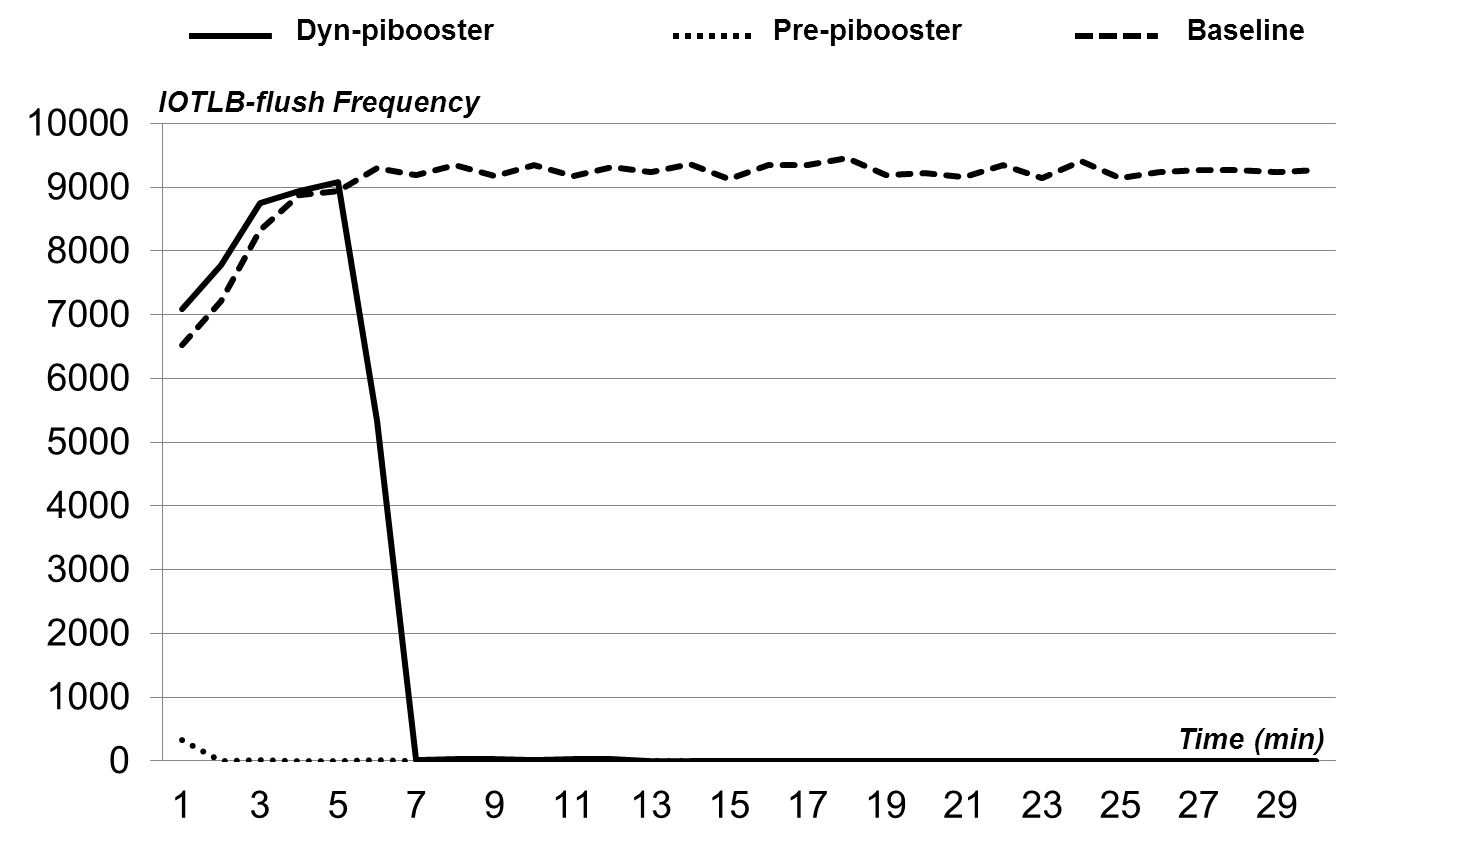
\includegraphics[scale=0.55]{image/iotlbflush.png} \\
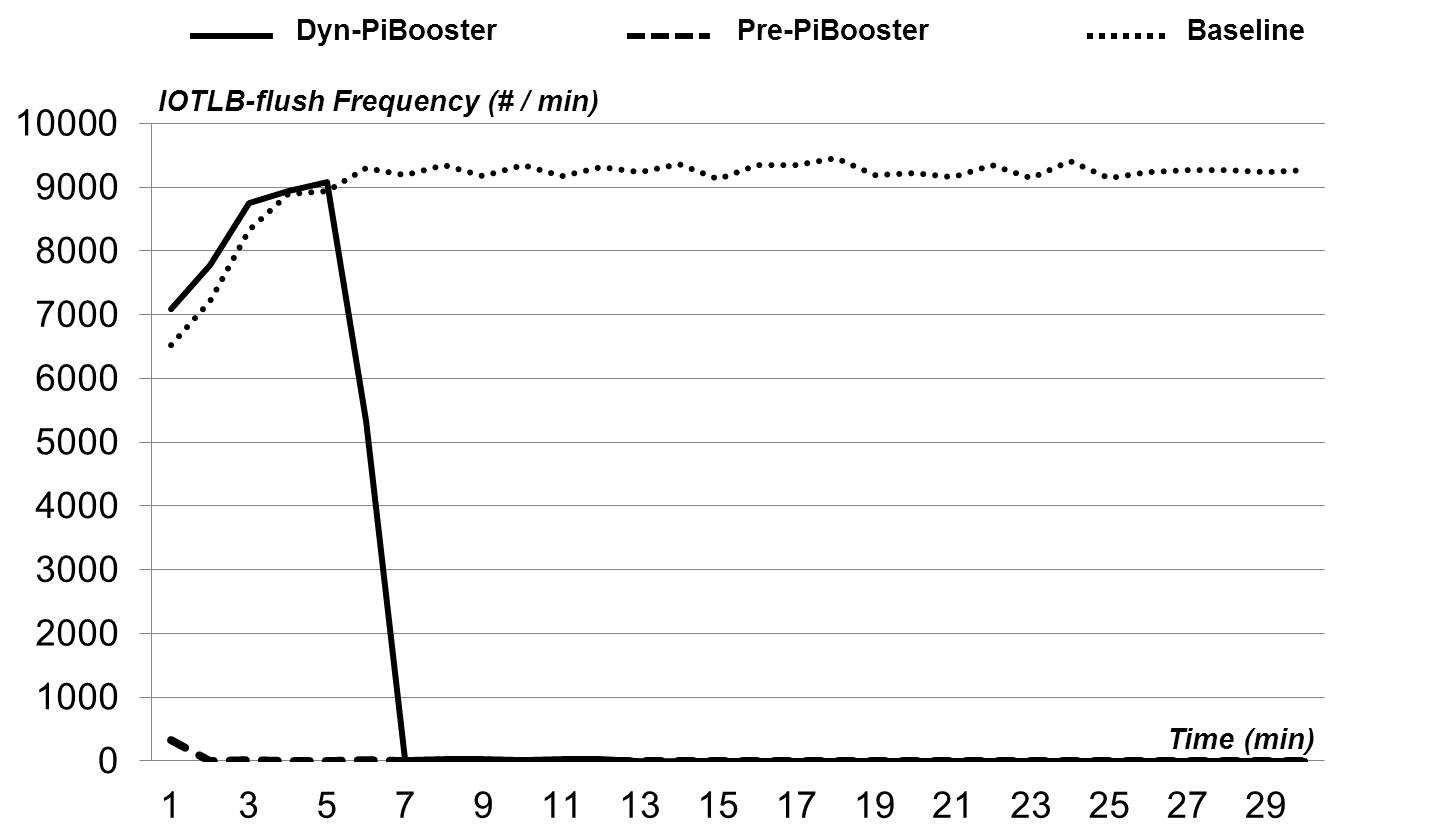
\includegraphics[width=0.5\textwidth]{image/micro/iotlbflush.jpg} \\
\caption{The frequency of IOTLB flushes.  In the \prename group the frequency is reduced from a very low level to zero within 1 minutes. In the \dynname group, the frequency drops sharply within two minutes from the high level to zero. Both control groups indicate that the \name could always enter the stable state (i.e., zero frequency).}
\label{fig:iotlbflush}
\end{figure}

\subsubsection{Frequency of IOTLB Flushes}
In this test, we aim to evaluate the effectiveness of the fine-grained validation on the addition IOTLB flushes.
We sample the frequency of the IOTLB flushes in 30 minutes.
The measurement results are illustrated in Figure~\ref{fig:iotlbflush}.
In the baseline group, the frequency of the IOTLB flushes is increasing in the first five minutes, and then keeps at a high flush rate until the test finishes.
In the \prename group, the flush frequency quickly decreases to zero level in about one minute and keeps at the level.
In the \dynname group, the flush frequency sharply decreases to zero when the \name is enabled. The \name roughly spends two minutes entering the stable state.
Thus, we can conclude that the fine-grained validation scheme is able to efficiently and effectively eliminate the IOTLB flushes introduced by the DMA validations.

%Y-axis represents the frequency of IOTLB-flush, corresponding to the time period (i.e., one minute) of x-axis for the first thirty minutes that the \emph{busy state} lasts. From this figure, frequency in the baseline group increases rapidly and remains stable five minutes later. By contrast, frequency in the pre-\name group drops to zero level in a very short time. It can be safely concluded that the fine-grained validation module proposed by \name does eliminate the IOTLB flushes caused by concurrent processes creations/exits. The dyn-\name group shows that the frequency also can be dropped to zero level very quickly even if the system is already in a \emph{busy state}.

\begin{figure*}[t!]
    \centering
    \begin{subfigure}[t]{0.5\textwidth}
        \centering
        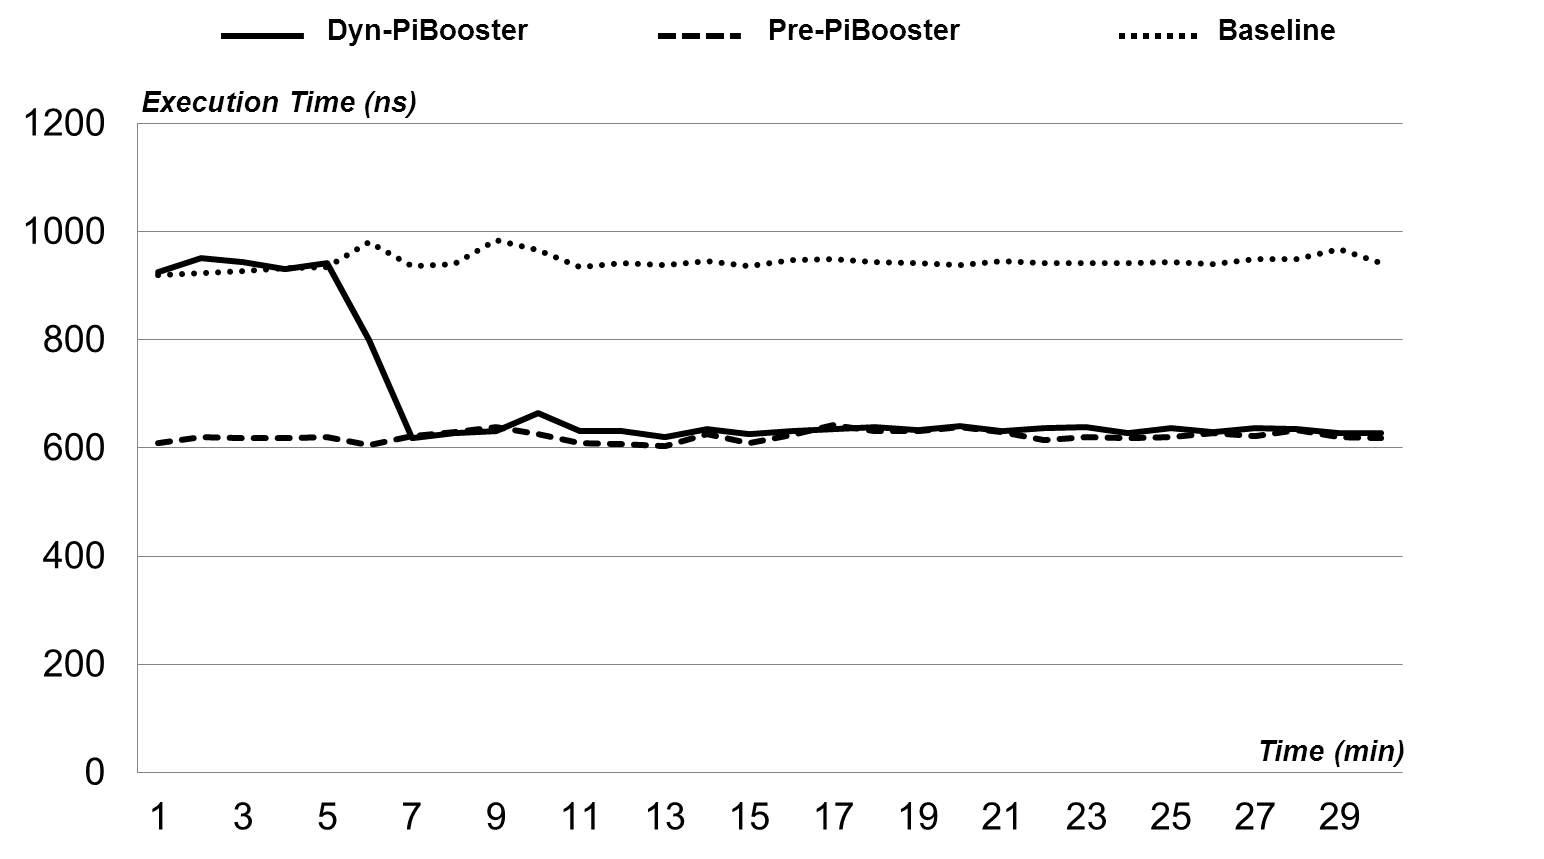
\includegraphics[height=2.0in]{image/micro/PGDalloc.png}
        \caption{Execution time of L1 allocation is improved by 34\%.}
        \label{fig:l1a}
    \end{subfigure}%
    ~
    \begin{subfigure}[t]{0.5\textwidth}
        \centering
        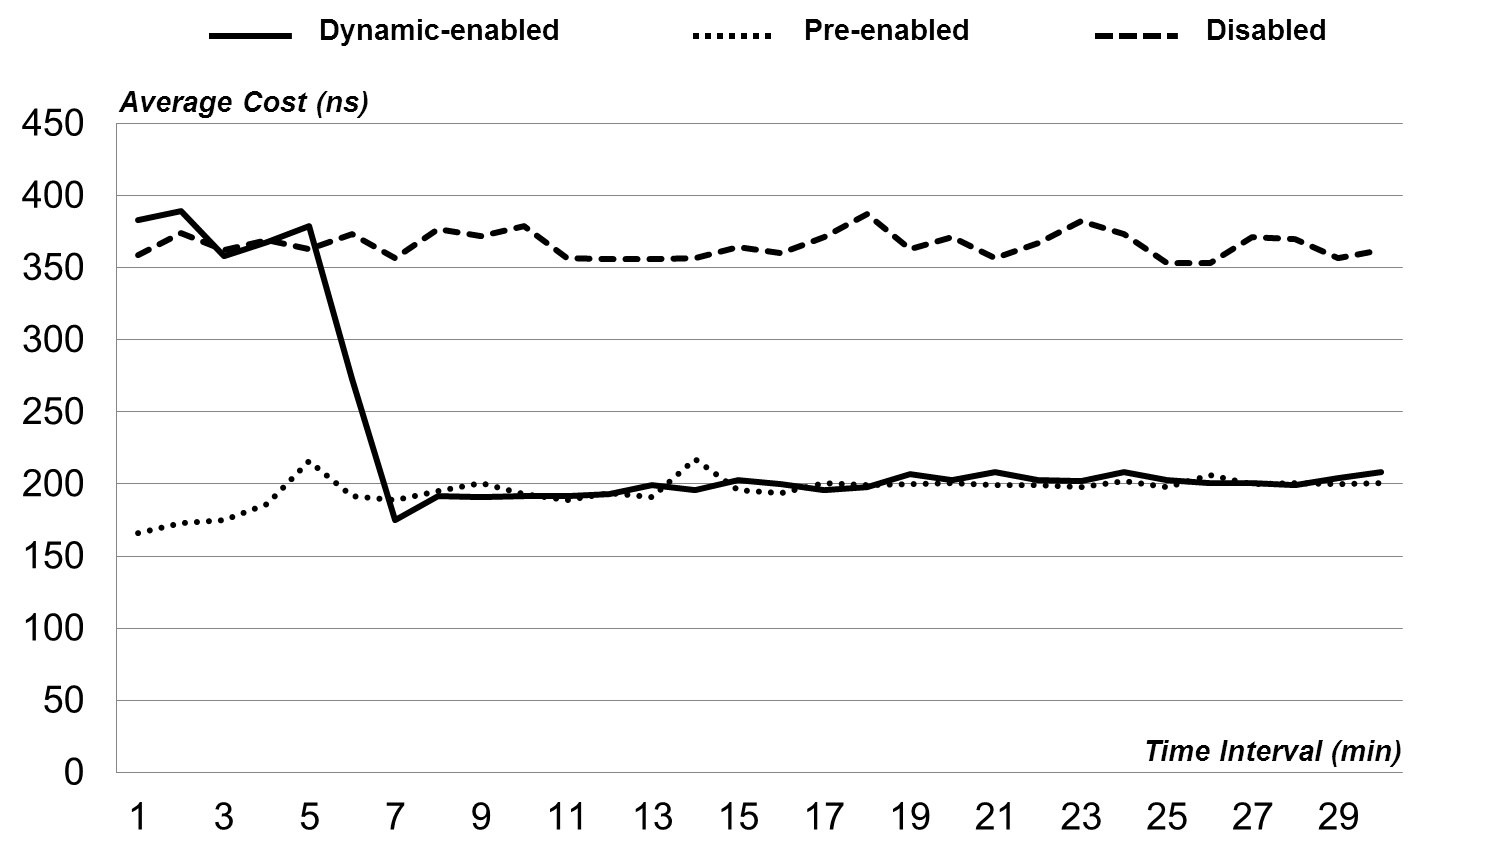
\includegraphics[height=2.0in]{image/micro/PGDfree.png}
        \caption{Execution time of L1 deallocation is improved by 47\%.}
        \label{fig:l1b}
    \end{subfigure}
    \caption{The execution time of L1 allocation and deallocation. The \name in the \dynname group can quickly enter the stable state in 2 minutes.}
    \label{fig:PGDtime}
\end{figure*}

\begin{figure*}[t!]
    \centering
    \begin{subfigure}[t]{0.5\textwidth}
        \centering
        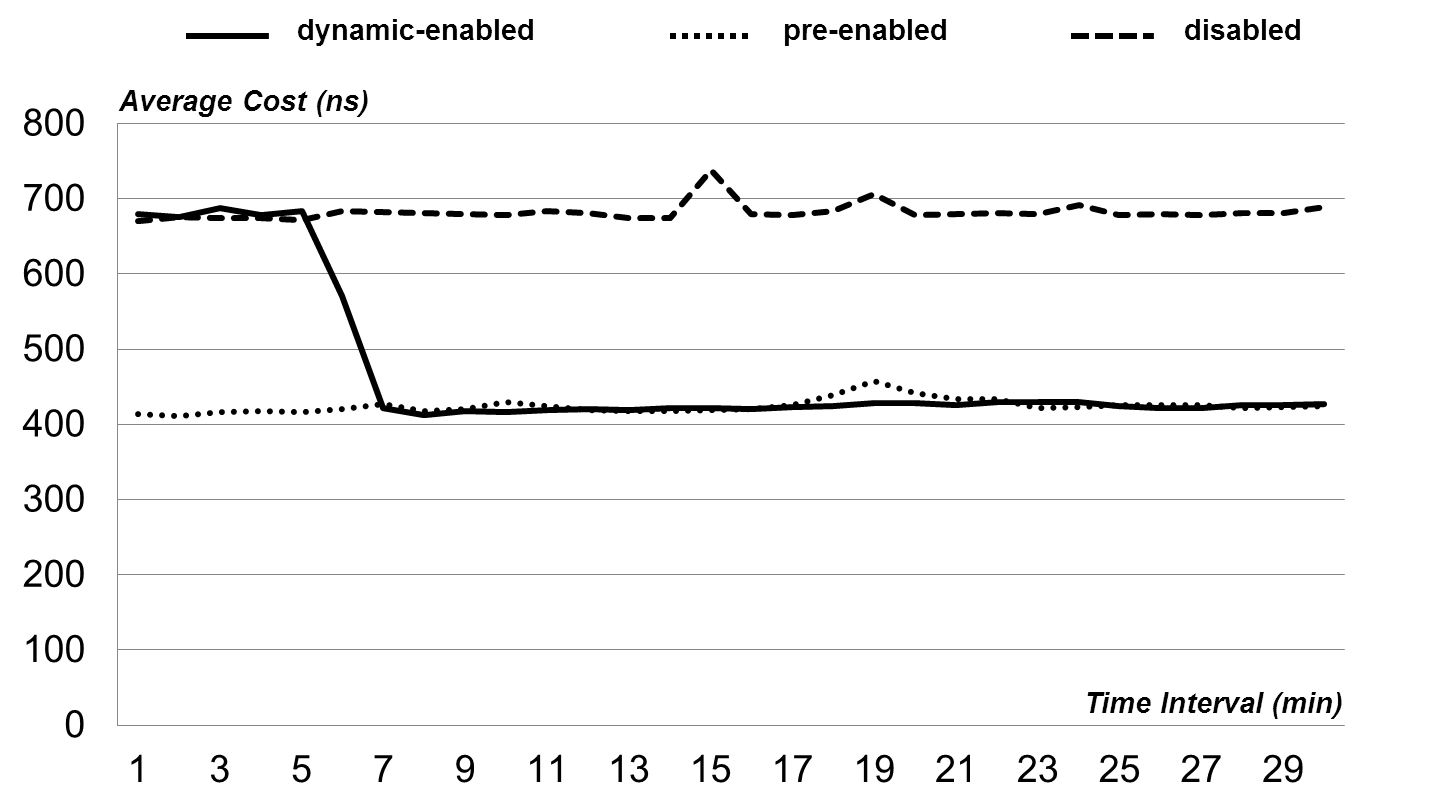
\includegraphics[height=2.0in]{image/micro/PMDalloc.png}
        \caption{Execution time of L2 allocation is improved by 38\%.}
        \label{fig:l2a}
    \end{subfigure}%
    ~
    \begin{subfigure}[t]{0.5\textwidth}
        \centering
        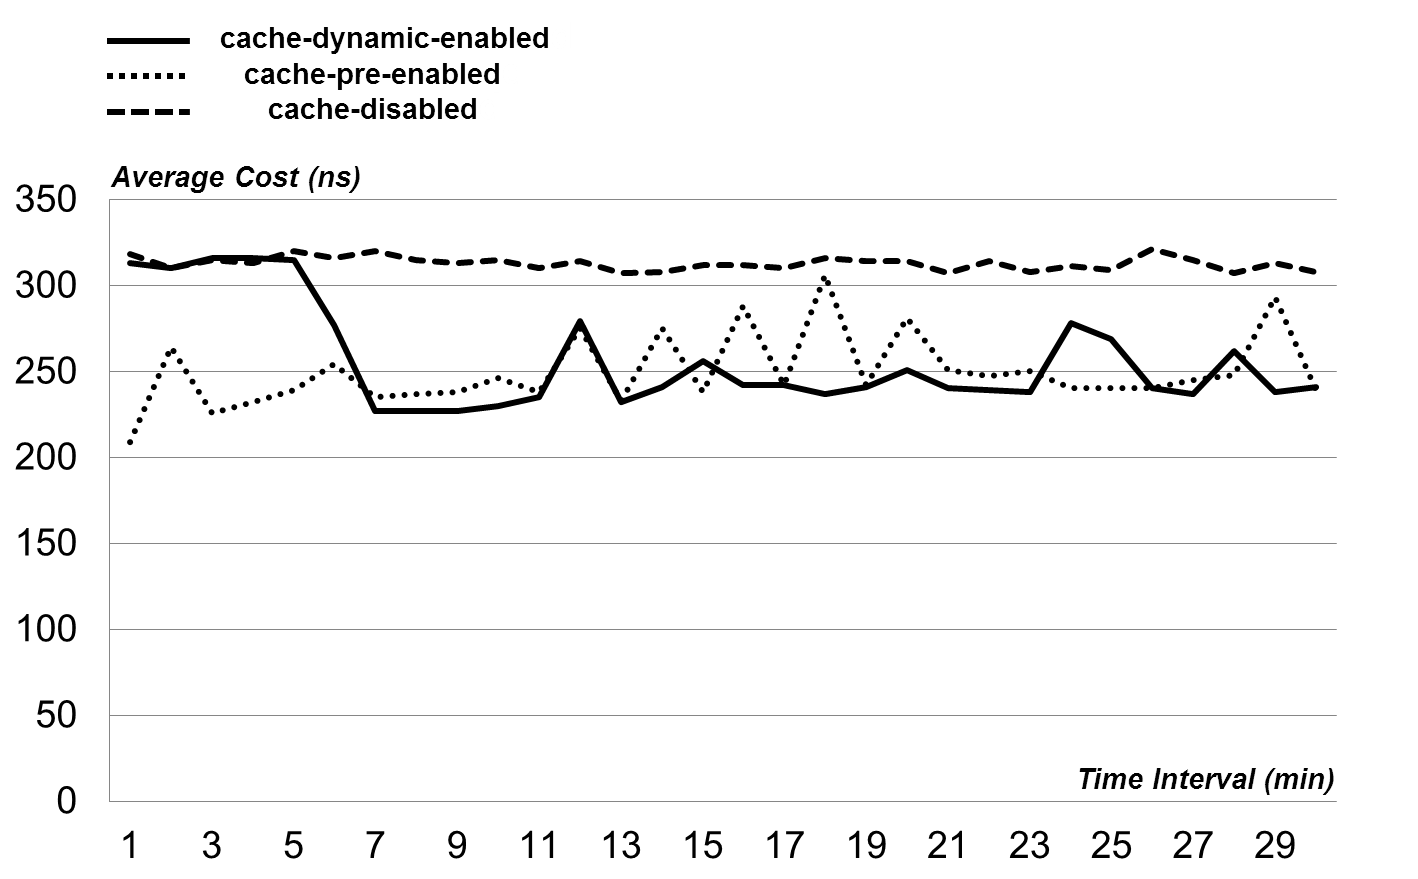
\includegraphics[height=2.0in]{image/micro/PMDfree.png}
        \caption{Execution time of L2 deallocation is improved by 22\%.}
        \label{fig:l2b}
    \end{subfigure}
    \caption{The execution time of L2 allocation and deallocation. The \name in the \dynname group can quickly enter the stable state in 2 minutes.}
    \label{fig:PMDtime}
\end{figure*}

\begin{figure*}[t!]
    \centering
    \begin{subfigure}[t]{0.5\textwidth}
        \centering
        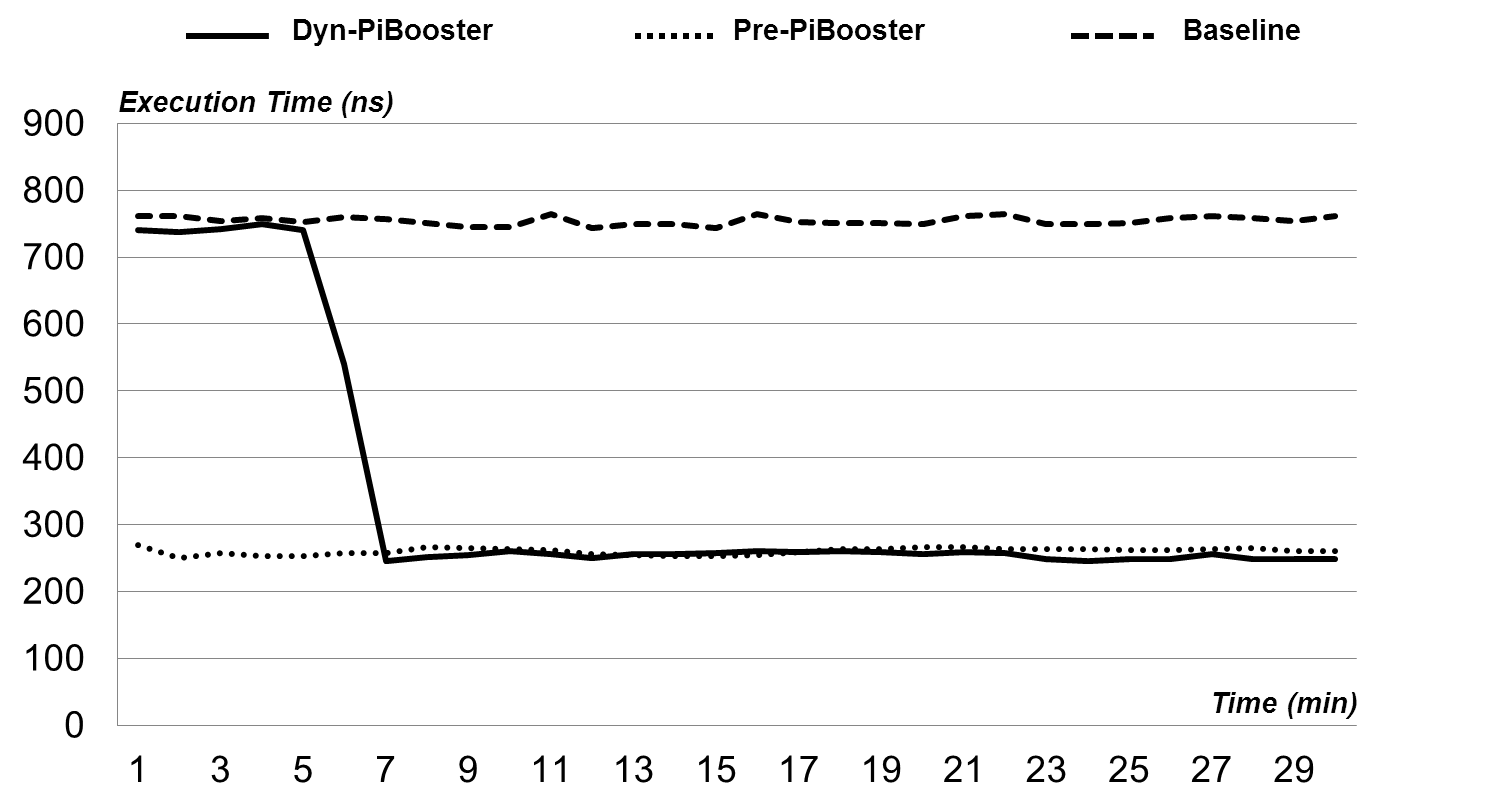
\includegraphics[height=2.0in]{image/micro/PTEalloc.png}
        \caption{Execution time of L3 allocation is improved by 65\%.}
        \label{fig:l3a}
    \end{subfigure}%
    ~
    \begin{subfigure}[t]{0.5\textwidth}
        \centering
        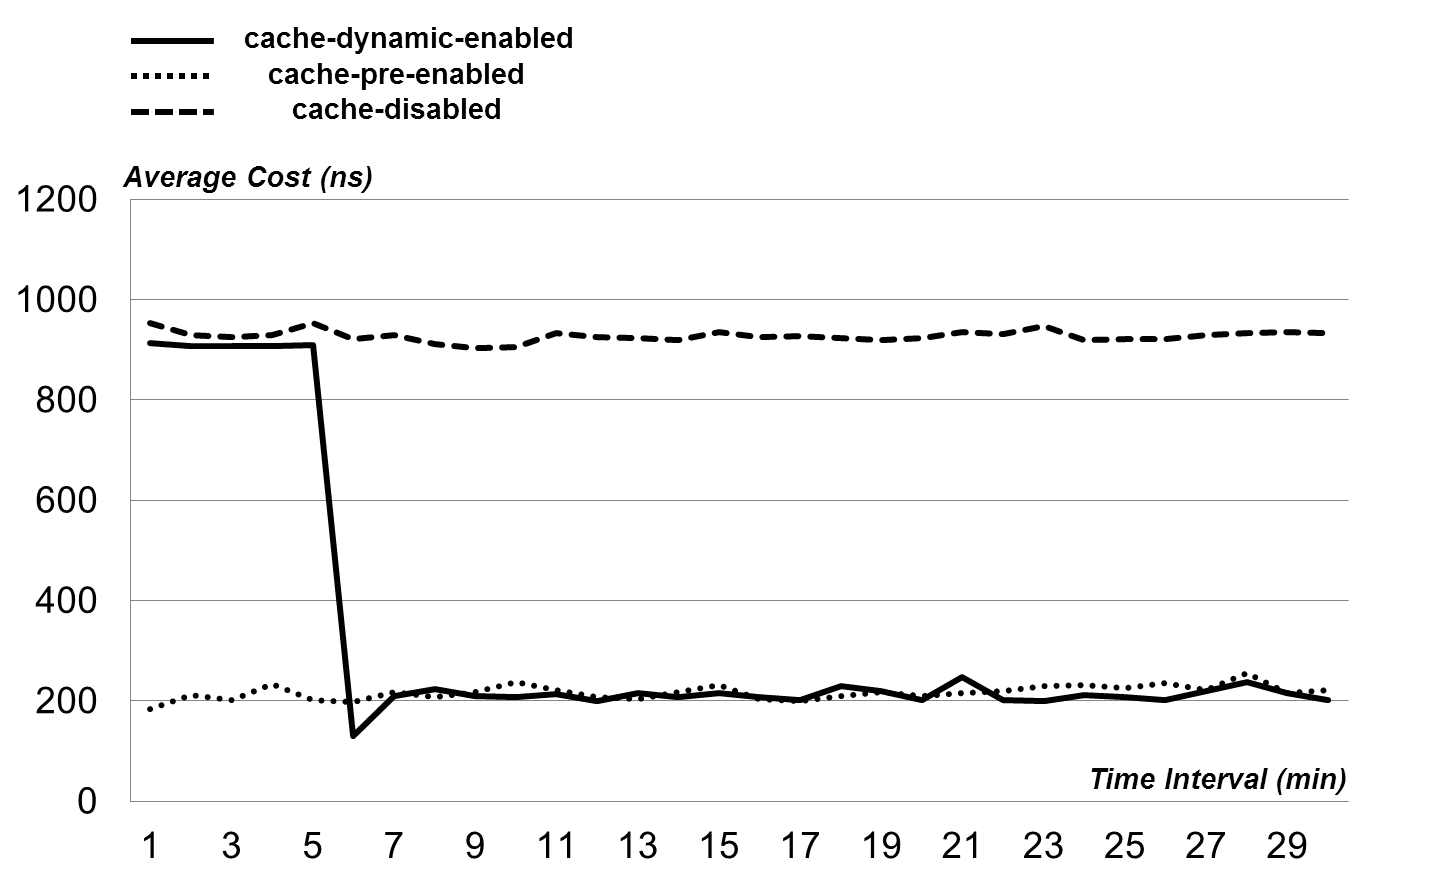
\includegraphics[height=2.0in]{image/micro/PTEfree.png}
        \caption{Execution time of L3 deallocation is improved by 65\%.}
        \label{fig:l3b}
    \end{subfigure}
    \caption{The execution time of L3 allocation and deallocation. The \name in the \dynname group can quickly enter the stable state in 2 minutes.}
    \label{fig:PTEtime}
\end{figure*}

\subsubsection{CPU Usage Measurement}
��As there are three levels of the guest page table, and each level has its (de)allocation functions, e.g., pgd\_alloc and pgd\_free for the L1 level.
In order to clearly observe the changes of the CPU usage, we measure them separately.
We continuously measure them in 30 minutes, and calculate the average execution time of each function in each one minute.
Note that in the \dynname group, we enable the \name 5 minutes after the workload starts to run.


As shown in Figure~\ref{fig:PGDtime}, \ref{fig:PMDtime}, and \ref{fig:PTEtime}, the execution time in the \prename group, for a pair of allocation and deallocation of the three-level page table, from top to bottom are (622, 196), (424, 242) (260,217) in nanoseconds, while in the baseline group, the corresponding execution time in nanoseconds are (944, 366), (682, 313), (755, 627). Accordingly, the improvements are (34\%, 47\%), (38\%, 22\%) and (65\%, 65\%).
%putting together
Putting them together, the page table allocations and deallocation can be improved by 45\% and 55\% on average respectively.
Note that the \name in the \dynname group can achieve the same performance improvement as the one in the \prename group.
The transitional stage to the stable state only needs less than 2 minutes, as illustrated in Figure~\ref{fig:PGDtime}, \ref{fig:PMDtime}, and \ref{fig:PTEtime}.

\mypara{The Worst Case}
With \name enabled, guest kernel firstly goes through the \cache for page table allocations. If the cached semi-writable pages cannot satisfy the requirements (a.k.a, cache miss), the \cache would have to allocate writable pages using the existing memory allocators following the traditional paths,.
In this case, the execution time is the traditional execution path plus the path in the \cache.
As a result, the execution time of the page table allocation is even longer than that of the baseline (Figure~\ref{fig:overview} (a)).
However, the overhead introduced by the \name path is negligible, as the control flow will immediately return when the list is empty.
More specifically, the overhead consists of the function innovation provided by the \emph{pop} interface, related stack adjustment and the checking of the cache list and the page type.
Putting them together, the overhead are less than 20 instructions.
Fortunately, the worst case does not often occur. According to our observations in the \dynname group, the number of the worst cases is $348$, out of $198990$ allocation requests in 30 minutes.
Note that the page-table deallocation is always completed successfully in a constant time.

%\zhi{In the pre-\name group, the probabilities of cache miss are 9/550 (1\% PGD), 38/2200(1\% PMD), 322/6633(4\% PTE),respectively. In the dyn-\name group, the probabilities of cache miss are 7/540 (1\% PGD), 24/2160(1\% PMD), 320/6333(5\% PTE),respectively.}

%When cache is pre-enabled, the ratio between the total pages in cache and the total pages as page tables is approximately equal to 1:1, which indicates that the cache mechanism takes up a small memory percentage of the stress tool.

\begin{table}[!ht]
\footnotesize
\begin{center}
\begin{tabular}{|l|l|l|}
\hline
{\textbf{Levels of Page Table}} & {\textbf{\prename (\#)}} & {\textbf{\dynname (\#)}} \\ \hline
L1 & $5$  & $4$ \\ \hline
L2 & $26$ & $20$ \\ \hline
L3 & $145$ & $136$ \\ \hline
Total & $176$ & $160$ \\ \hline
\end{tabular}
\end{center}
\caption{Cache usages in both groups of \prename and \dynname are small, occupying 176 pages and 160 pages, respectively.}
%And the memory size of cached pages only takes up to 0.2\% of the tool's memory.
\label{tab:PGpool}
\end{table}

\subsubsection{Memory Usage Measurement}
Besides CPU usage, we also measured the memory consumption of the \cache.
To clearly see the page usage in each level, we measured the cached page numbers in three levels and results are listed in Table \ref{tab:PGpool}.
In the \prename group the \cache has $5$, $26$ and $145$ semi-writable pages ready for allocations, totally occupying $704KB$, which is quite similar to the \dynname group, where the cache has $160$ in total, occupying memory $640KB$. As a result, the \cache in both groups consume an insignificant memory usage, always less $1MB$.
%Also note that the conditions of freeing pages in cache in the dyn-\name group heavily rely on a specific scenario, which may not work for other situations. We will further discuss the conditions in future work.

%And the reason why the dyn-\name group has fewer cached pages than that of the pre-\name group is that a certain number of page table pages has been freed to the memory allocator before the \name is enabled.



\subsection{Macro-Benchmarks}
The purpose of the macro-benchmarks is to evaluate the effects of \name on the overall system.
All measurements are divided into two groups: 1) the baseline group with the default settings, and 2) the \name group with the \name enabled.

\begin{figure}[htp]
\centering
%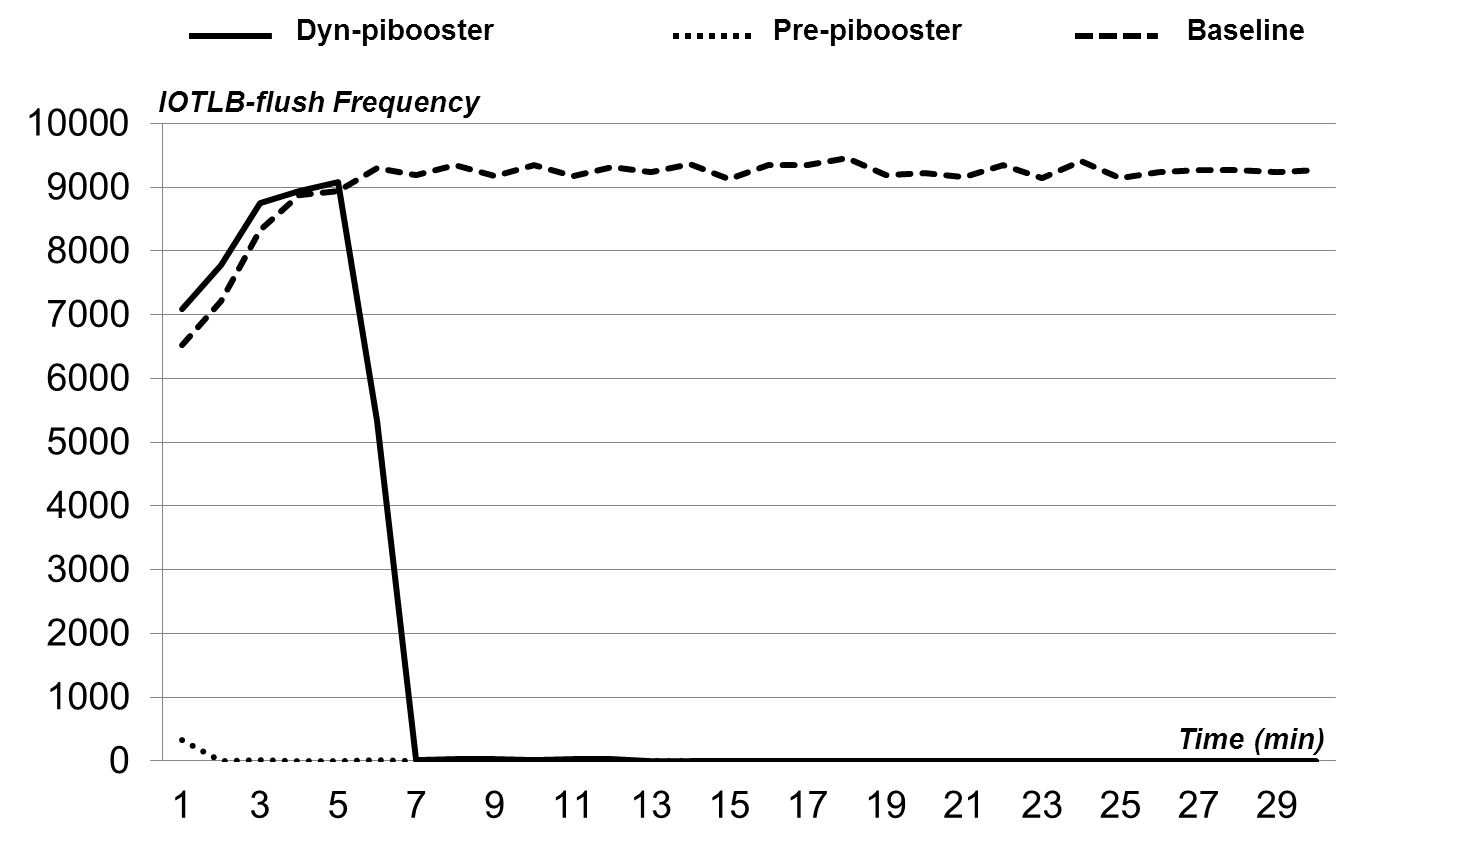
\includegraphics[scale=0.55]{image/iotlbflush.png} \\
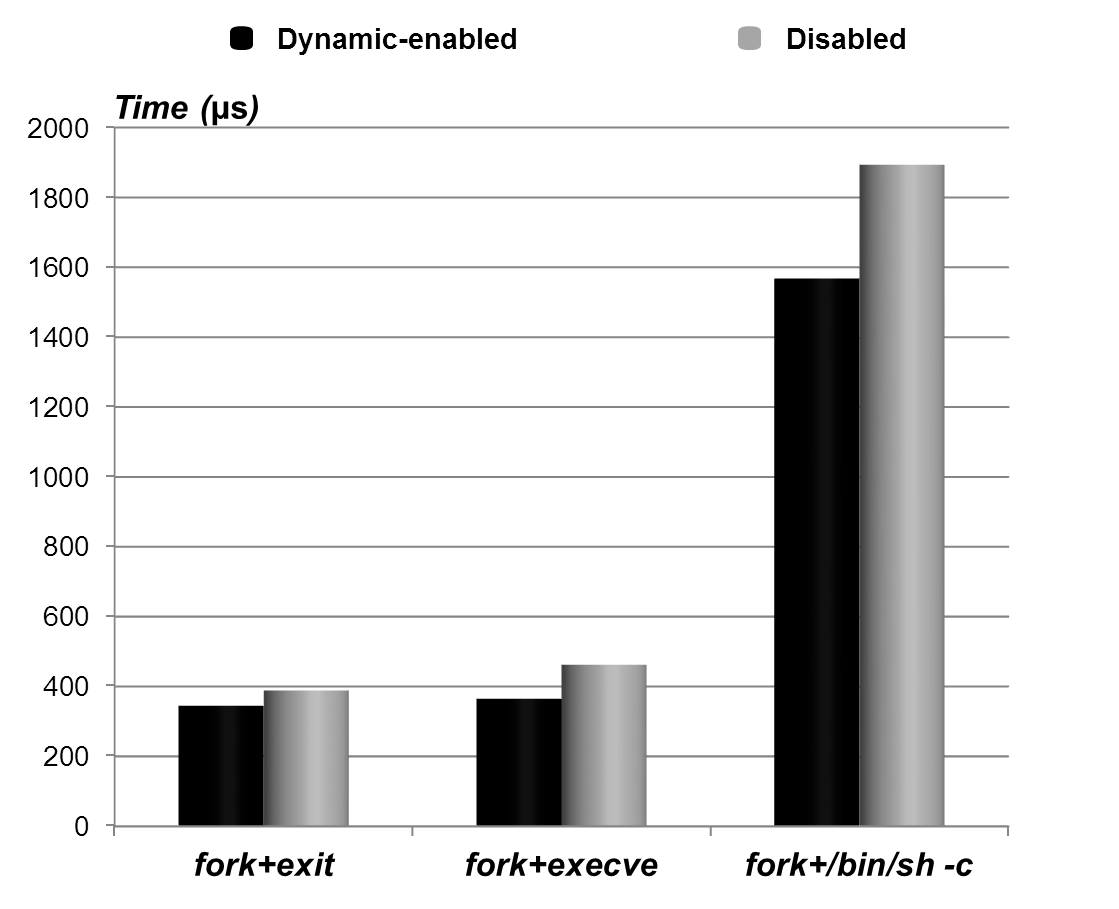
\includegraphics[width=0.4\textwidth]{image/macro/lmbench.png} \\
\caption{The execution time on average in the \name group is reduced by 11\%, 17\% and 21\%, from left to right.}
\label{fig:lmbench}
\end{figure}

\subsubsection{Latency Improvements in Process Creations and Exits}
Lmbench is a macro-benchmark tool for measuring the latency of the process creations and exits (i.e., fork+exit, fork+execve, fork+/bin/sh -c), shown in Figure~\ref{fig:lmbench}.
The Lmbench are configured using the default parameters, except for the parameters of processor MHz and memory range.
In our experiment platform, the CPU frequency is $3.2$ GHz, memory range is set as $1024$ MB to save measurement time.
As illustrated in Figure~\ref{fig:lmbench}, the processes of \emph{fork+exit}, \emph{fork+execve} and \emph{fork+/bin/sh -c} in the \name group costs $344$, $365$, and $1567$ in microseconds, $11$\%, $17$\%, $21$\% faster than the ones in the baseline group.
We believe that the improvement will significantly benefit the workloads that rely on many short-time temporary processes.

\begin{figure}[htp]
\centering
%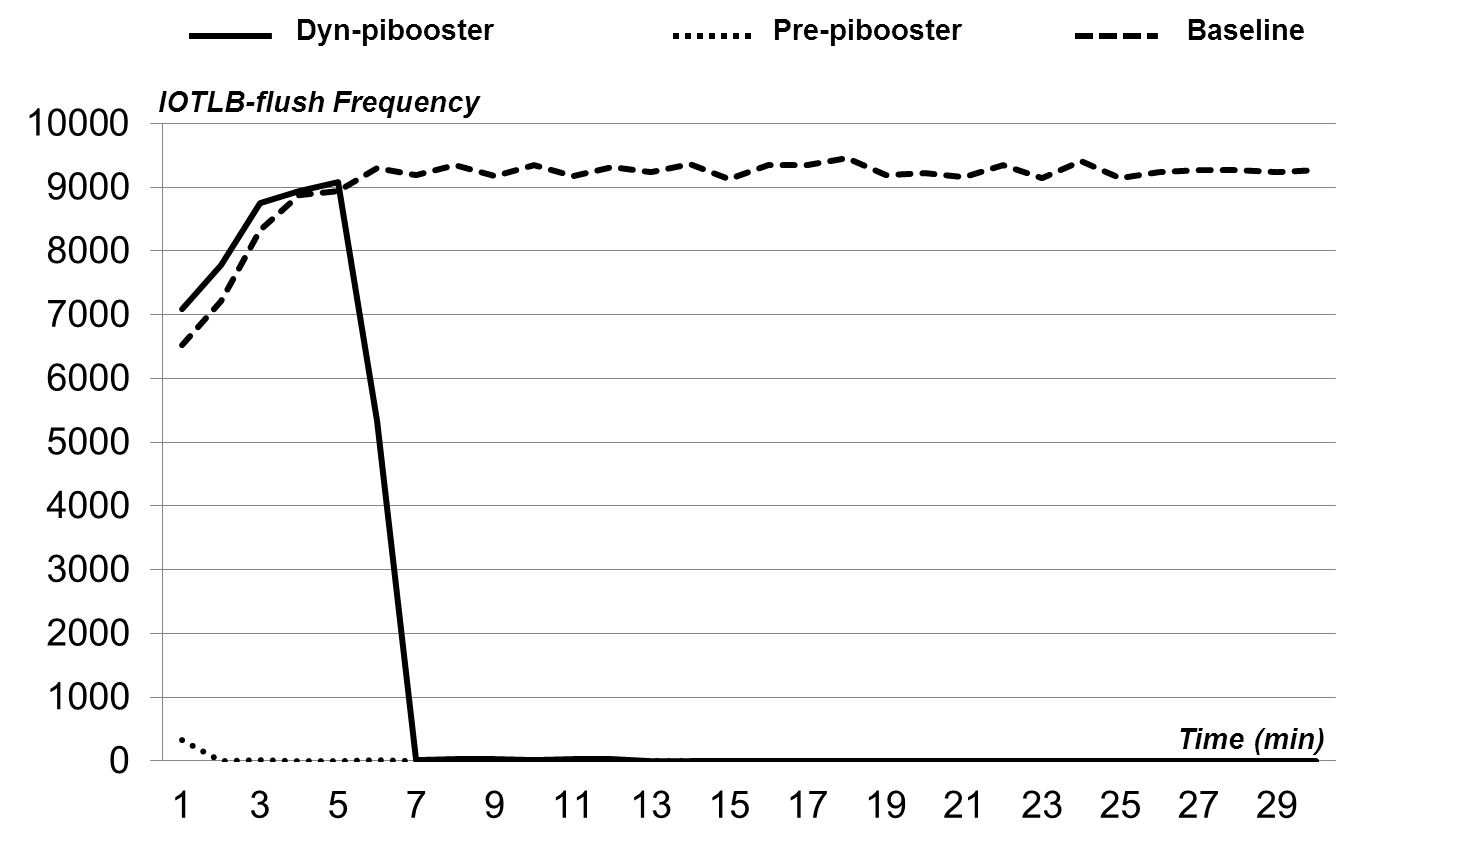
\includegraphics[scale=0.55]{image/iotlbflush.png} \\
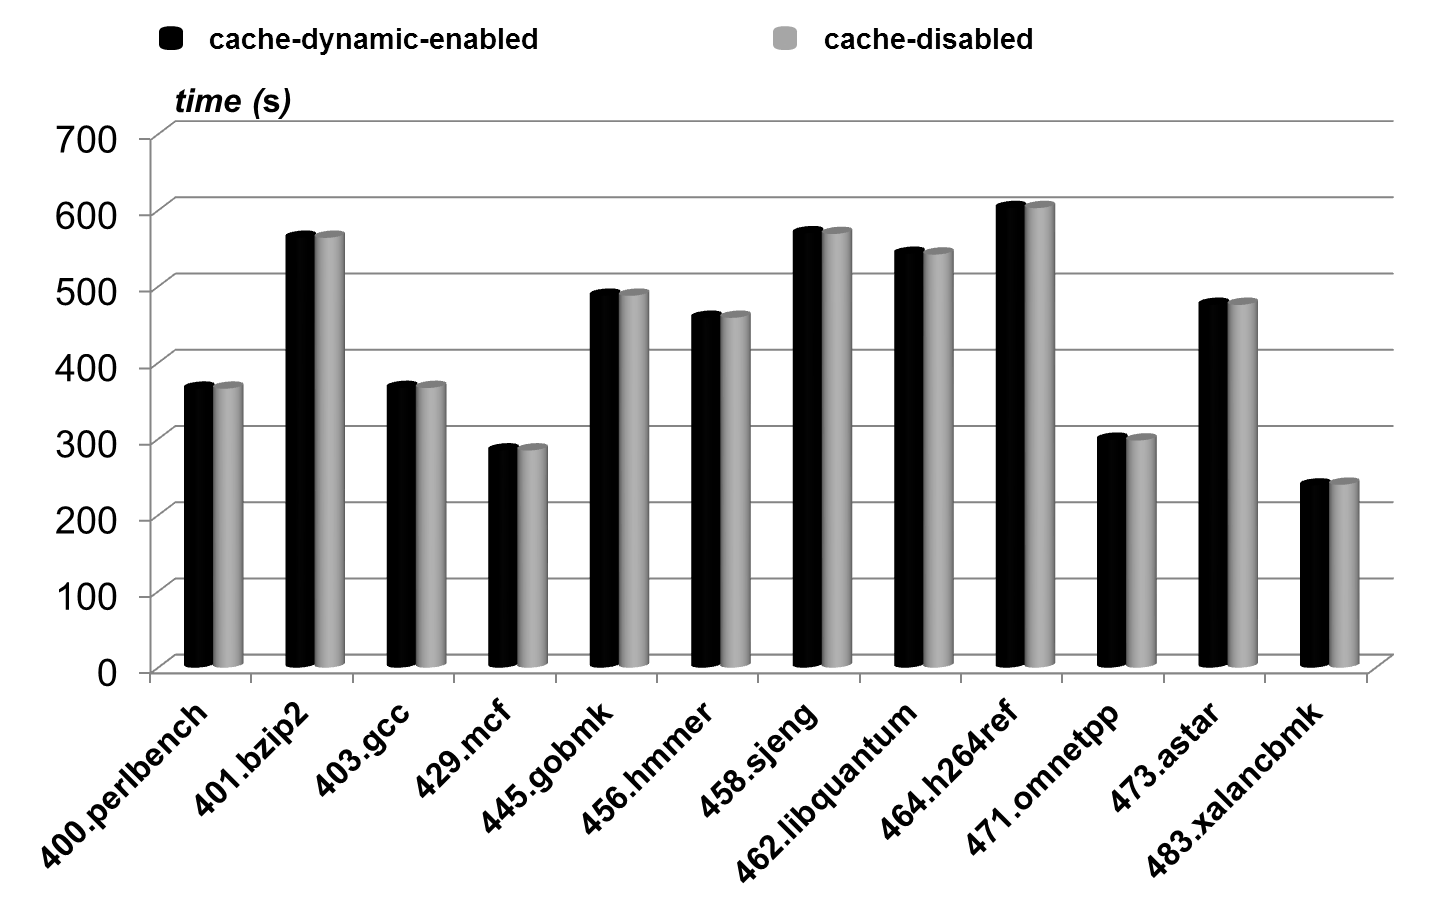
\includegraphics[width=0.5\textwidth]{image/macro/spec.png} \\
\caption{The differences among all the benchmarks are within 0.42\%, indicating that the \name has no negative effect on system performance.}
\label{fig:spec}
\end{figure}

\subsubsection{SPECINT}
SPEC CINT2006~\cite{specint} is an industry standard benchmark intended for measuring the performance of the CPU and memory.
In our experiment, the tool version is SPECint 2006 v1.2, which has $12$ benchmarks in total and they are all invoked with the configuration file \emph{linux64-ia32-gcc43+.cfg}.
All measurement results are listed in Figure~\ref{fig:spec}.
Among the benchmarks, the time differences between the baseline group and the \name group are very small, e.g., the maximum difference is within 0.42\%, which is produced by the \emph{483.xalancbmk}.
All of them produce the same or a little better performance results, indicating the \name has no negative effect on system performance.

\subsubsection{I/O Performance Measurements}
As we know, IOTLB is used to accelerate the DMA address translation to achieve better performance for I/O devices.
Therefore, if there are many IOTLB misses caused by frequent IOTLB flushes will introduce negative effects on the  I/O performance.
However,  rIOMMU~\cite{malka2015riommu} claims that the overhead caused by walking the IOMMU page tables due to IOTLB misses is so negligible that cannot be measured in the \emph{netperf}, because the main latency induced by I/O interrupt processing and the TCP/IP stack is several orders of magnitude larger than that of walking the page tables.
In addition, Nadav Amit \emph{et al.}~\cite{amit2012iommu} also has similar statements.
% that the IOTLB misses cannot be observed under regular circumstances, since the I/O memory (un)mapping operations consume much more time than that of the corresponding DMA transaction.

In this paper, we test the network I/O and disk I/O performances under regular circumstances.
%, and use these experiments as the revisiting of the problem between the IOTLB misses and I/O performance.
We measured the network I/O using \emph{netperf} tool. Specifically, we have two machines that are directly connected through the Ethernet cable.
The client on one machine set a bulk of TCP packets to the server on another machine. Note that emulated workload is also enabled on the client machine to trigger IOTLB flushes.
The sending buffer is $16KB$ and the test lasts 60 seconds.
The measurement results are listed in Table~\ref{tab:netperf}.
By comparing both values of $\mu$ and $\sigma$, we find that there is no detectable negative effect on the network I/O.
Similarly, we also test the disk I/O using lmbench. The results indicate that the disk I/O speed remains the same.
The above two experiments also as new evidences to support the observations in ~\cite{amit2012iommu, malka2015riommu}.

\begin{table}[!ht]
\footnotesize
\begin{center}
\begin{tabular}{|l|l|l|}
\hline
{\textbf{Throughput (\emph{Mbps})}} & {\textbf{\name}} & {\textbf{Baseline}}    \\ \hline
Range & $87.880-88.010$ & $87.880-87.950$ \\ \hline
Arithmetic Mean ($\mu$)  &  $87.926$ & $87.913$ \\ \hline
Standard Deviation ($\sigma$) &  $0.028$ & $0.021$ \\ \hline
\end{tabular}
\end{center}
\caption{The netperf results of network I/O indicate that the overhead introduced by the IOTLB misses is negligible.}
\label{tab:netperf}
\end{table}

In fact, it is suggested that the overhead introduced by the IOTLB misses can be measured by using a high-speed I/O device (i.e., Intel's I/O Acceleration Technology~\cite{lauritzenintel}) so as to do DMA copy operations in a pseudo pass-through mode of IOMMU~\cite{amit2012iommu}. The experiment results indicate that DMA-copy speed is largely reduced by the IOTLB misses.
Moshe Malka \emph{et al.} use rIOMMU with ibverbs library~\cite{ibverbsevaluation,kerr2011dissecting} to establish a high-performance setting in order to measure the cost of one IOTLB miss.

We believe that the \name can effectively reduce the overhead in the above high-speed settings, and we also plan to conduct experiments in the future.
%However, currently we do not have a machine with the Intel I/O acceleration technology. Thus, we have to postpone this experiment. 

%play an important role in I/O environments requiring high performance, which will be evaluated in our future work by utilizing the previous approaches and the I/O high-speed device.
%Both studies aim to create high performance settings that reduce the DMA transactions to the magnitude of $\upmu$s so that IOTLB becomes the dominant factor.


%\begin{figure}[htp]
%\centering
%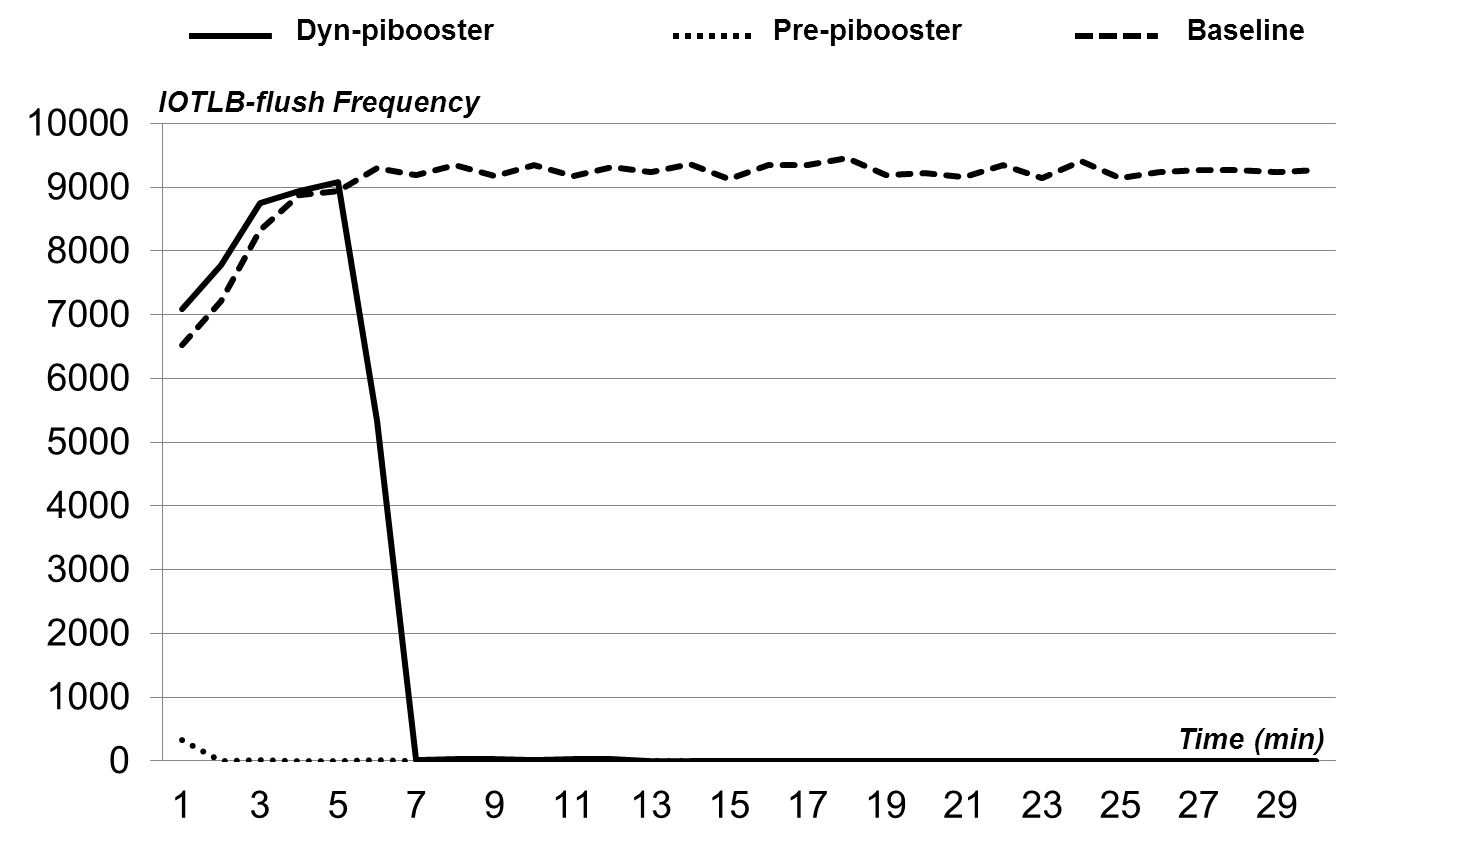
\includegraphics[scale=0.55]{image/iotlbflush.png} \\
%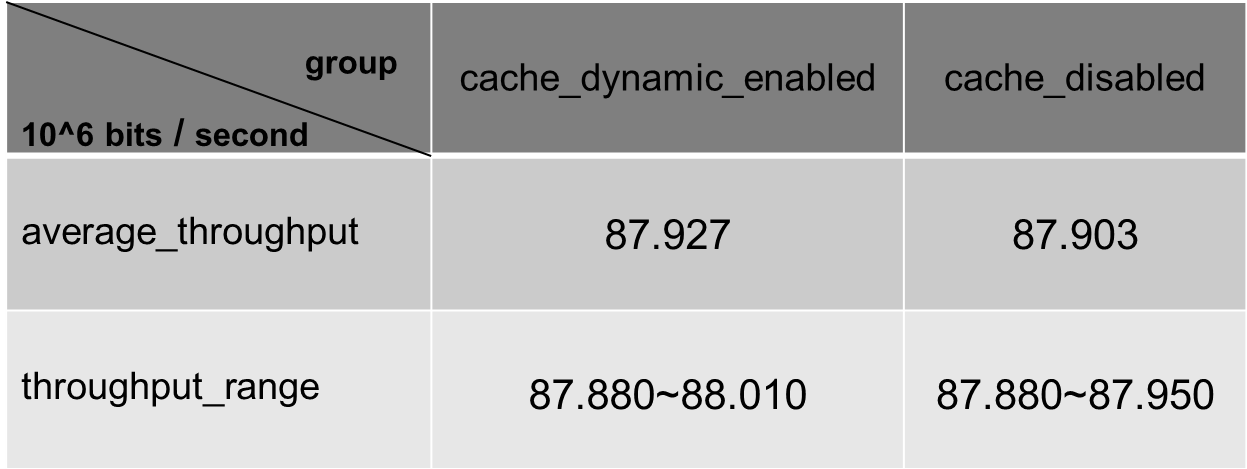
\includegraphics[width=0.5\textwidth]{image/macro/netperf.png} \\
%\caption{Netperf}
%\label{fig:netperf}
%\end{figure}
%|p{1.7cm}|p{1.8cm}|p{1.7cm}


%\begin{figure*}[!t]
%\centering
%\subfigure[PGD Alloc]{
%\label{fig:subfig:a}
%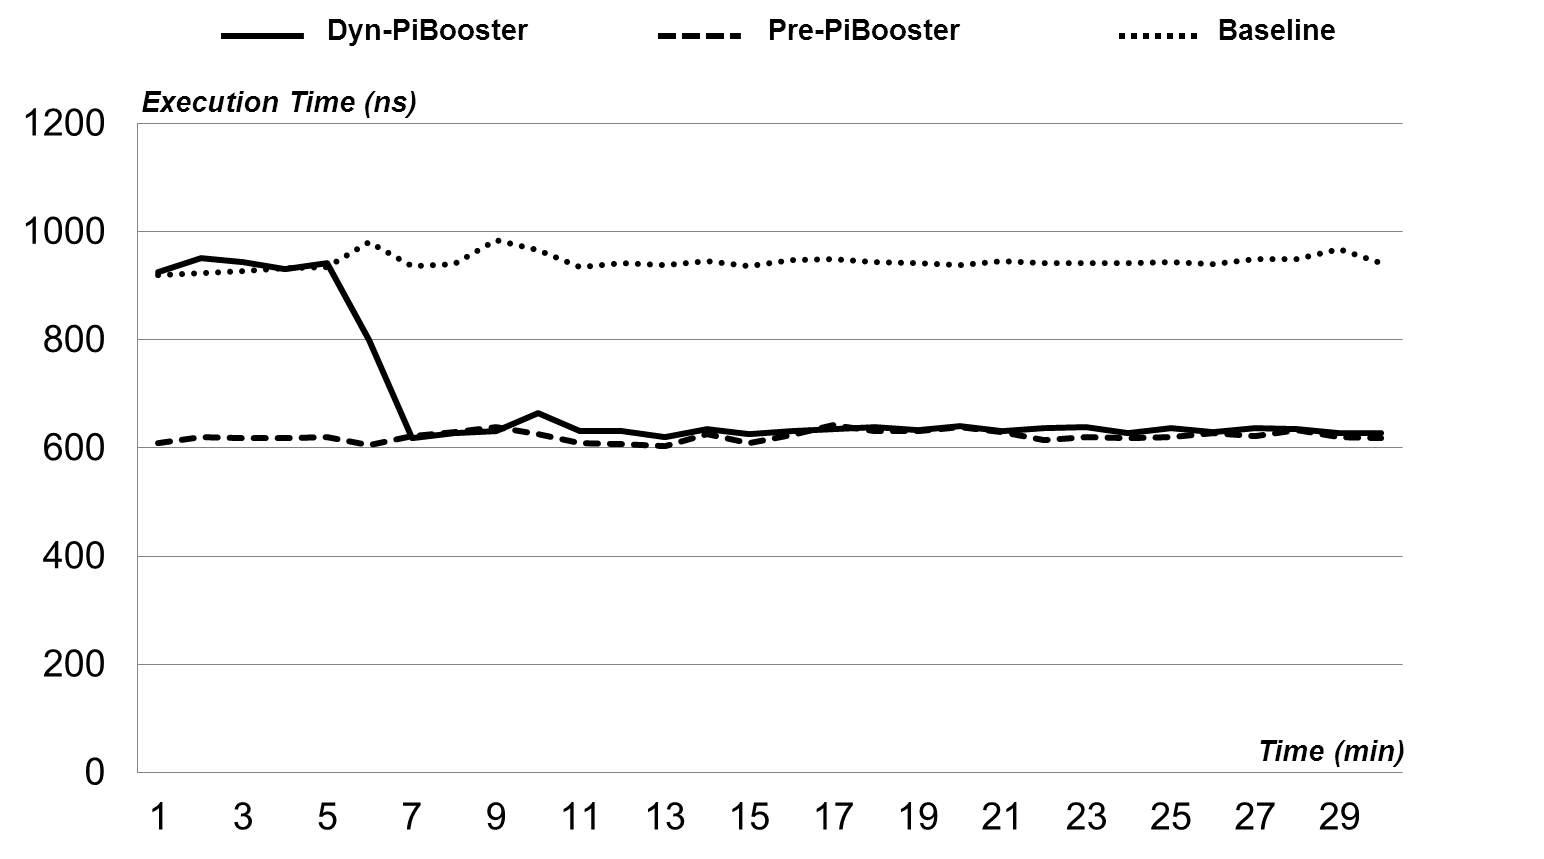
\includegraphics[width=0.5\textwidth]{image/micro/PGDalloc.png}}
%\hspace{1in}
%\subfigure[PGD Free]{
%\label{fig:subfig:b}
%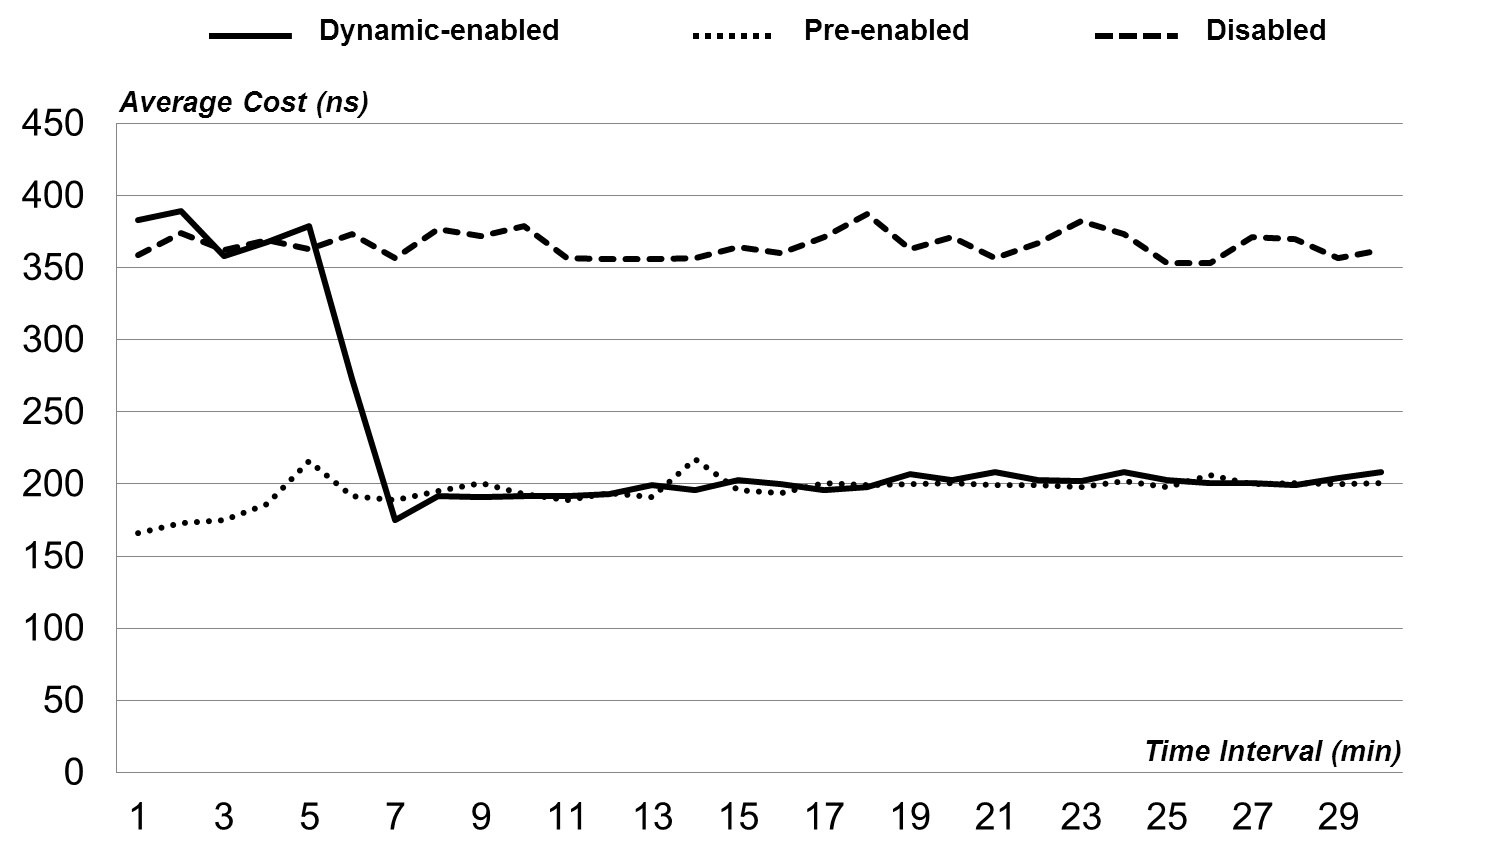
\includegraphics[width=0.5\textwidth]{image/micro/PGDfree.png}}
%\caption{Both page-table cache groups costs much less CPU cycles}
%\label{fig:PGDtime} %% label for entire figure
%\end{figure*}

%\begin{figure}
%\centering
%\subfigure[PGD]{
%\label{fig:subfig:a}
%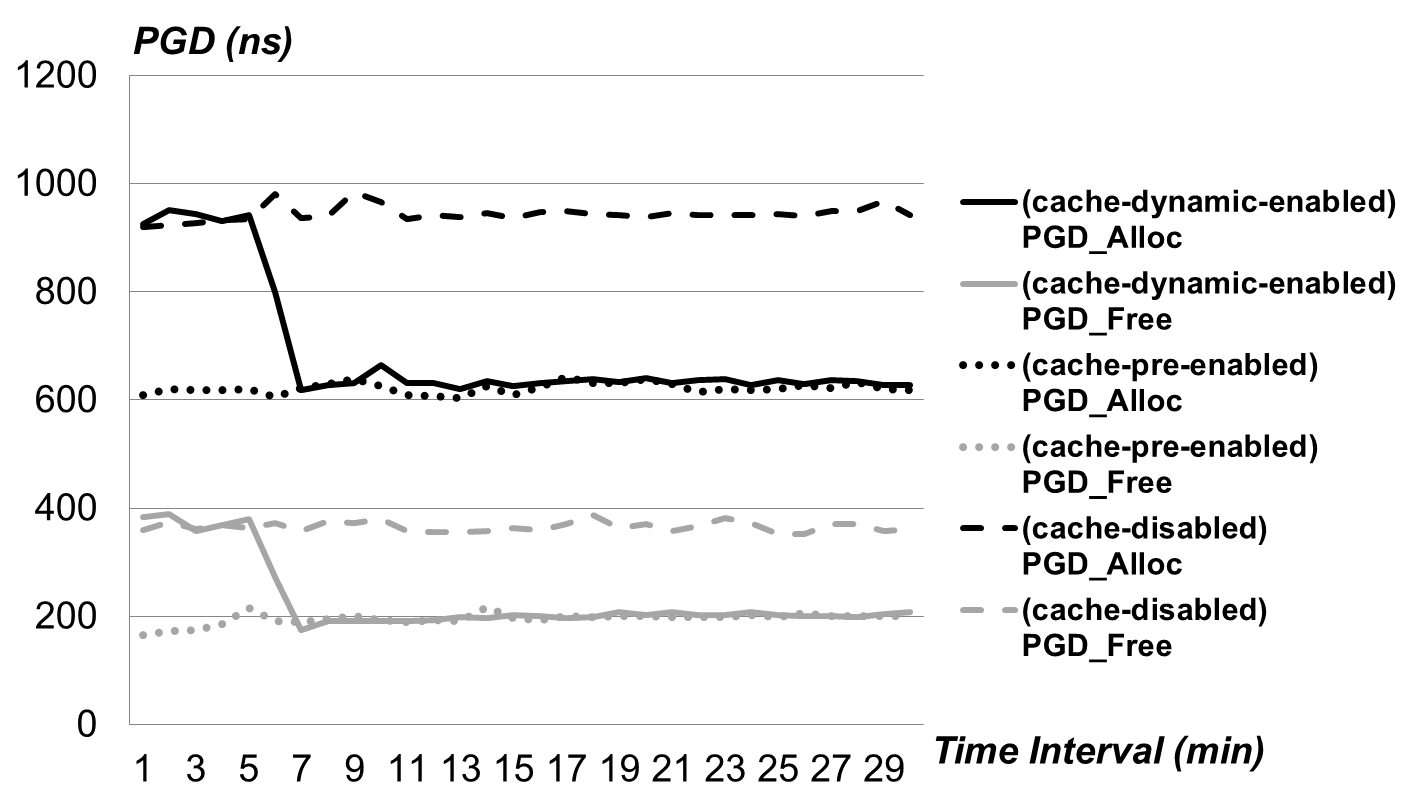
\includegraphics[width=0.5\textwidth]{image/micro/PGDtime.png}}
%\hspace{1in}
%\subfigure[PMD]{
%\label{fig:subfig:b}
%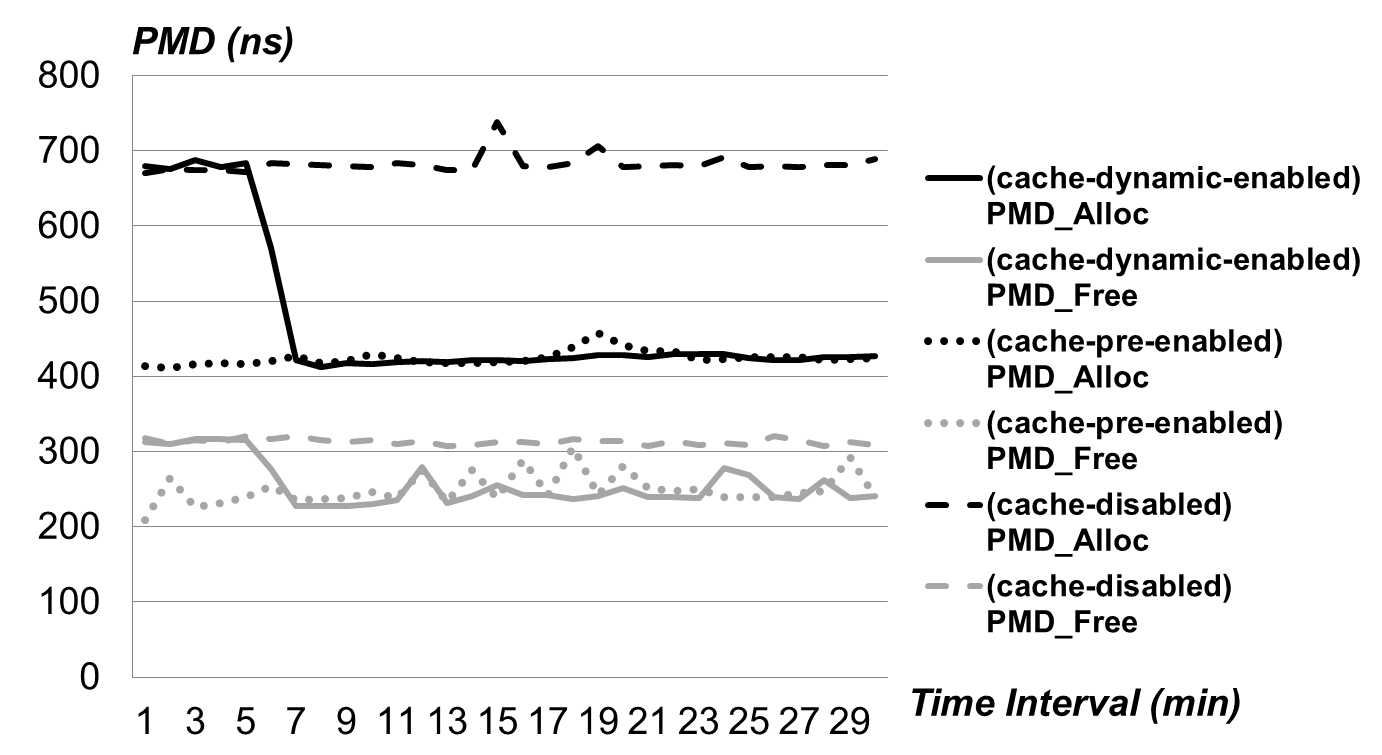
\includegraphics[width=0.5\textwidth]{image/micro/PMDtime.png}}
%\hspace{1in}
%\subfigure[PTE]{
%\label{fig:subfig:c}
%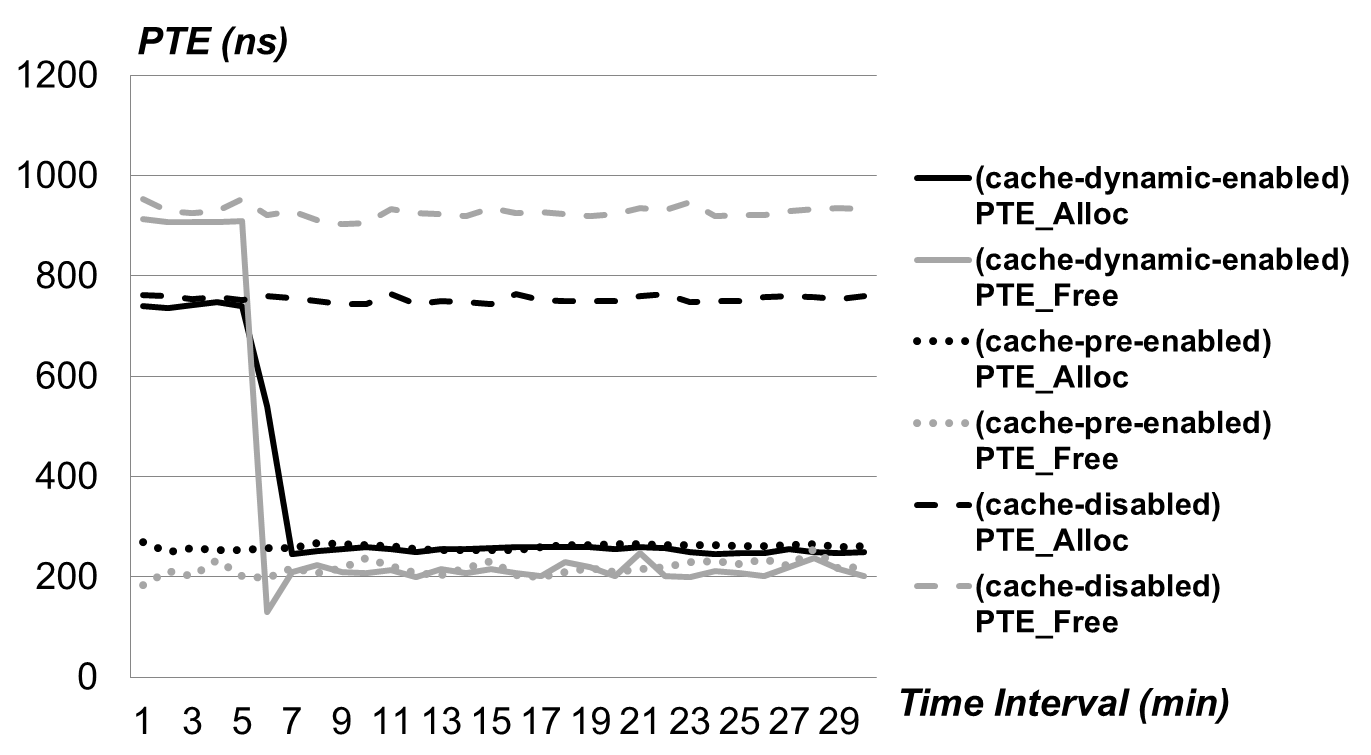
\includegraphics[width=0.5\textwidth]{image/micro/PTEtime.png}}
%\caption{CPU Usage for Each Level of Page Table}
%\label{fig:PGtime} %% label for entire figure
%\end{figure}

%\begin{figure}
%\centering
%\subfigure[PGD]{
%\label{fig:subfig:a}
%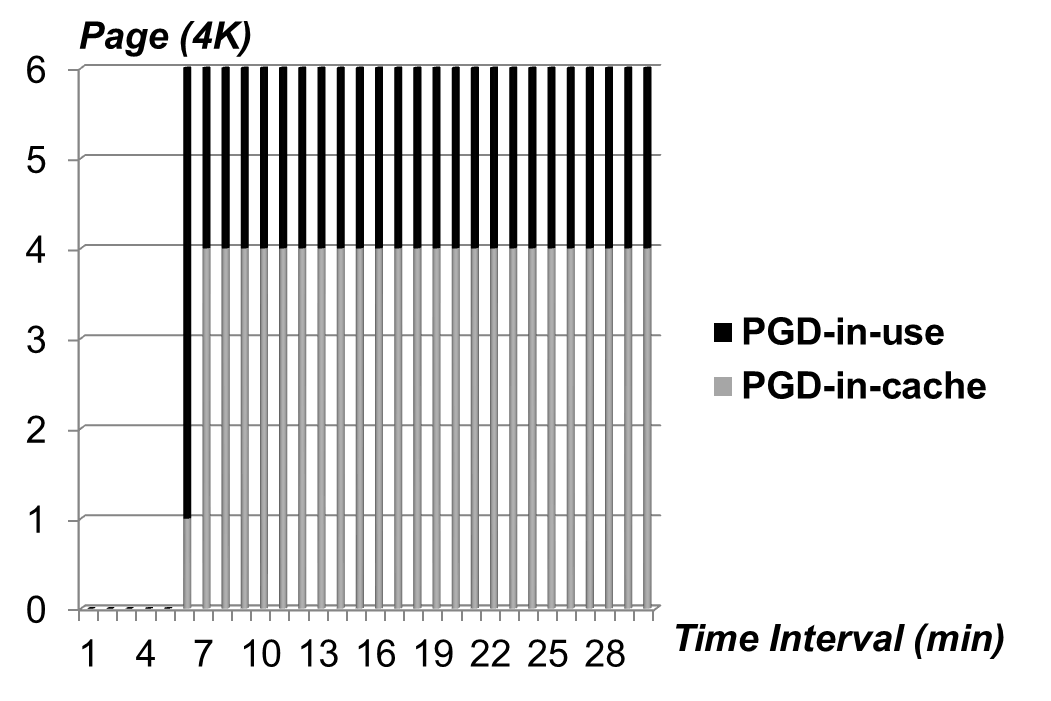
\includegraphics[width=0.5\textwidth]{image/micro/dyn_PGDpool.png}}
%\hspace{1in}
%\subfigure[PMD]{
%\label{fig:subfig:b}
%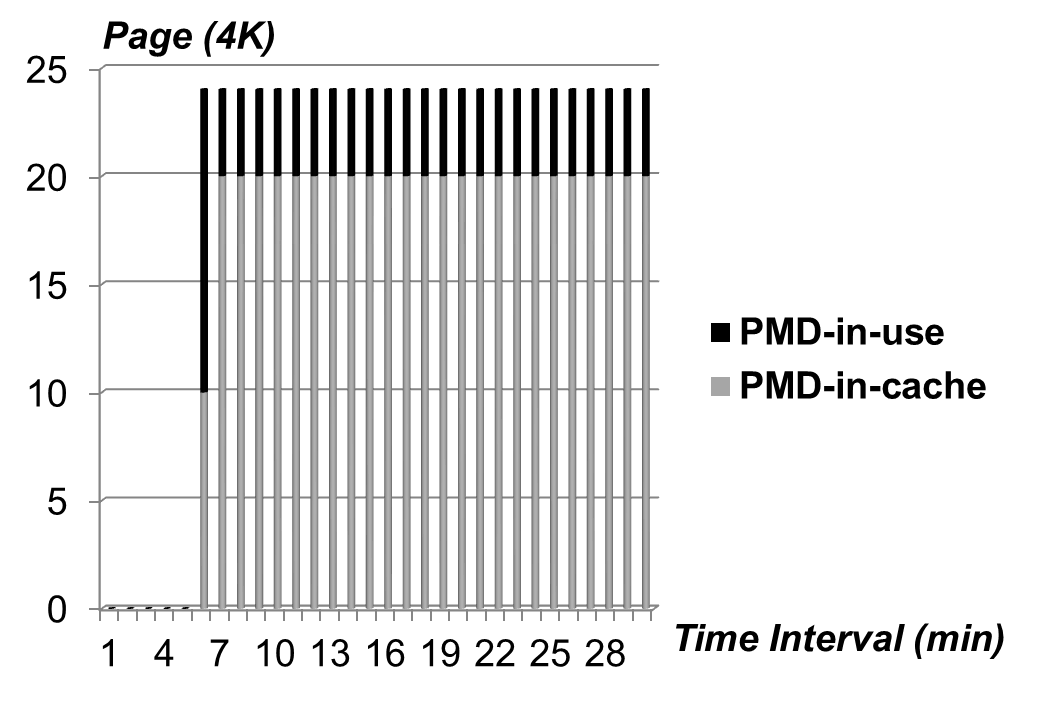
\includegraphics[width=0.5\textwidth]{image/micro/dyn_PMDpool.png}}
%\hspace{1in}
%\subfigure[PTE]{
%\label{fig:subfig:c}
%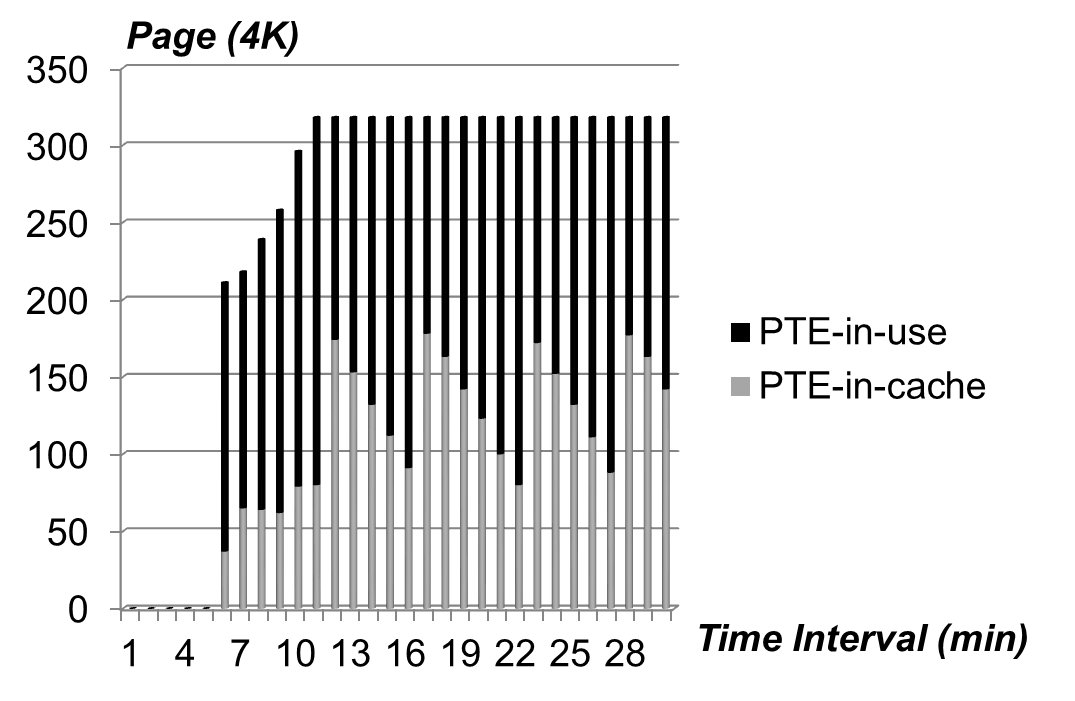
\includegraphics[width=0.5\textwidth]{image/micro/dyn_PTEpool.png}}
%\caption{Cache Pools Size for Cache-Dynamic-Enabled Group}
%\label{fig:dynPGpool} %% label for entire figure
%\end{figure}

%\begin{figure}
%\centering
%\subfigure[PGD]{
%\label{fig:subfig:a}
%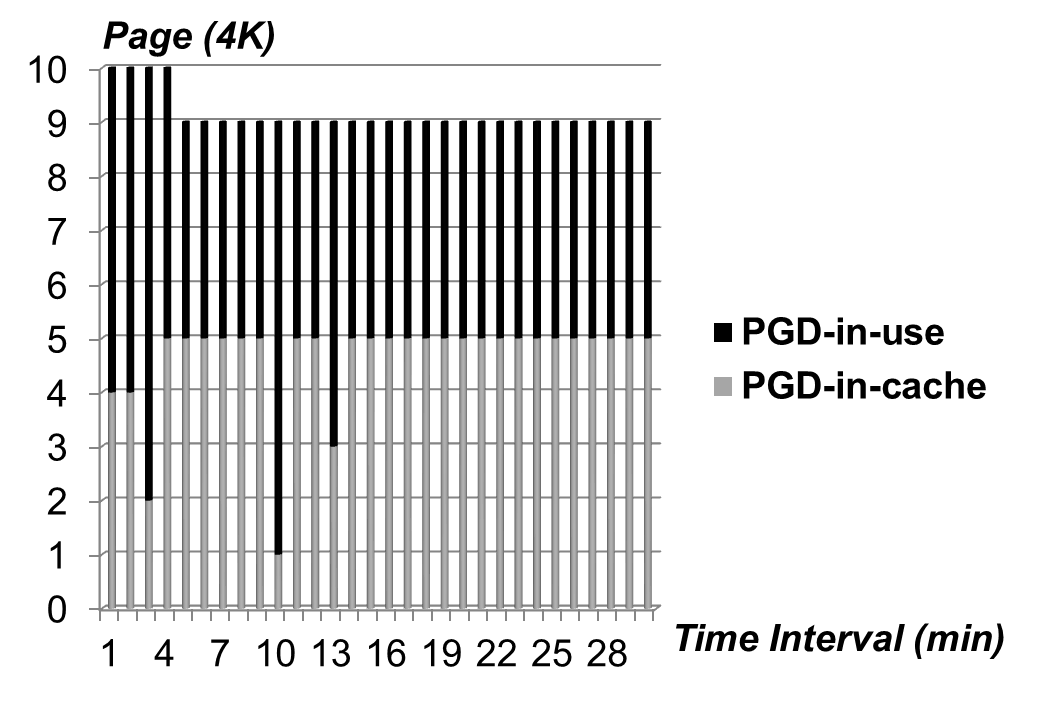
\includegraphics[width=0.5\textwidth]{image/micro/pre_PGDpool.png}}
%\hspace{1in}
%\subfigure[PMD]{
%\label{fig:subfig:b}
%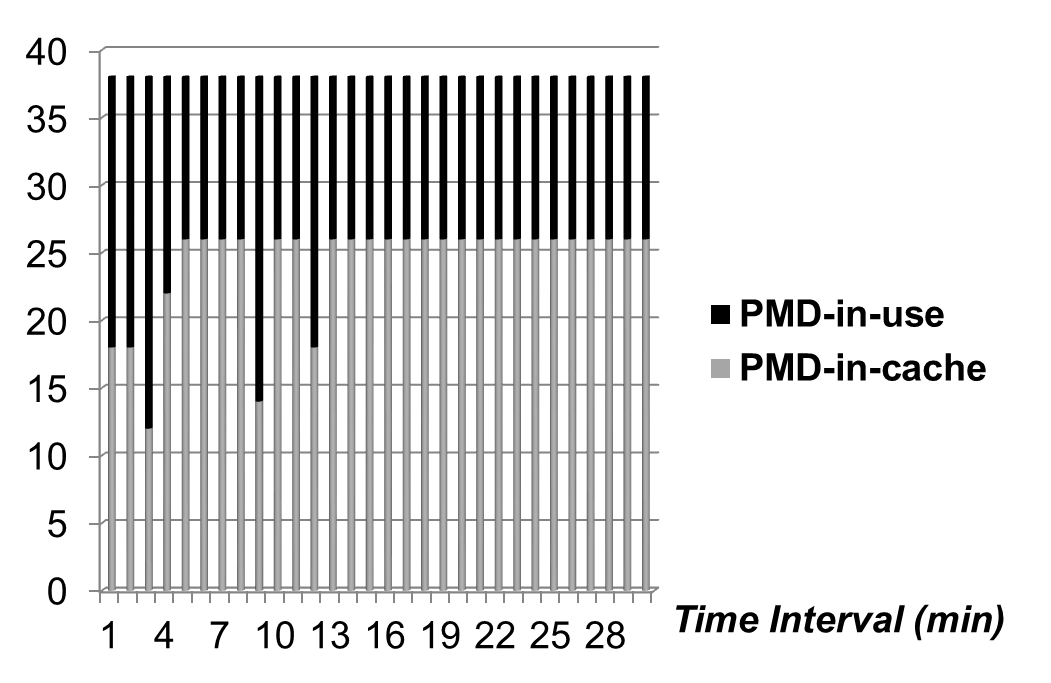
\includegraphics[width=0.5\textwidth]{image/micro/pre_PMDpool.png}}
%\hspace{1in}
%\subfigure[PTE]{
%\label{fig:subfig:c}
%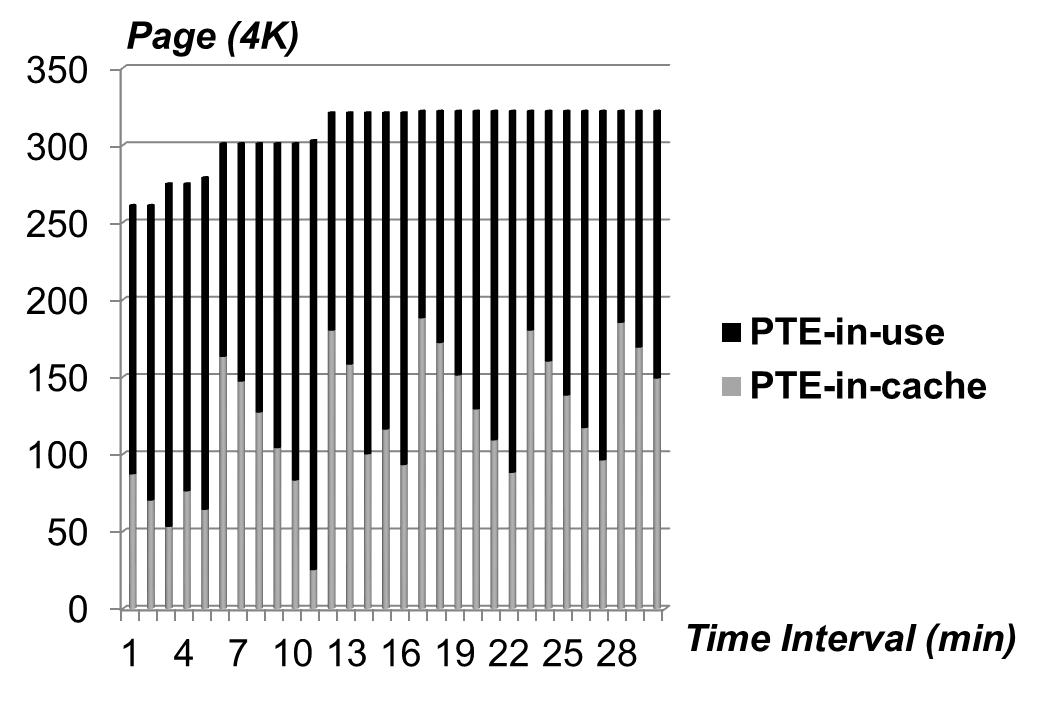
\includegraphics[width=0.5\textwidth]{image/micro/pre_PTEpool.png}}
%\caption{Cache Pools Size for Cache-Pre-Enabled Group}
%\label{fig:prePGpool} %% label for entire figure
%\end{figure}

%PGD & $5$  & $4$   & $>1:1$ \\ \hline
%PMD & $26$ & $12$   & $>2:1$ \\ \hline
%PTE & $145$ & $177$ & $<1:1$ \\ \hline
%Total & $176$ & $193$ & $<1:1$ \\ \hline

%PGD & $4$  & $2$   & $2:1$ \\ \hline
%PMD & $20$ & $4$   & $5:1$ \\ \hline
%PTE & $136$ & $182$ & $<1:1$ \\ \hline
%Total & $160$ & $188$ & $<1:1$ \\ \hline
%\begin{table}[!ht]
%\footnotesize
%\begin{center}
%\begin{tabular}{|l|l|l|}
%\hline
%{\textbf{Levels of Page Table}} & {\textbf{Semi-writable Page (\#)}} & {\textbf{Page-Table Page (\#)}} \\ \hline
%L1 & $5$  & $4$ \\ \hline
%L2 & $26$ & $12$ \\ \hline
%L3 & $145$ & $177$ \\ \hline
%Total & $176$ & $193$ \\ \hline
%\end{tabular}
%\end{center}
%\caption{The memory usage of the \cache is small in the \prename group, only occupying 176 pages. }
%And the memory size of cached pages only takes up to 0.2\% of the tool's memory.
%\label{tab:prePGpool}
%\end{table}

%\begin{table}[!ht]
%\footnotesize
%\begin{center}
%\begin{tabular}{|l|l|l|}
%\hline
%{\textbf{Levels of Page Table}} & {\textbf{Semi-writable Page (\#)}} & {\textbf{Page-Table Page (\#)}} \\ \hline
%L1 & $4$  & $2$ \\ \hline
%L2 & $20$ & $4$  \\ \hline
%L3 & $136$ & $182$ \\ \hline
%Total & $160$ & $188$ \\ \hline
%\end{tabular}
%\end{center}
%\caption{}
%\label{tab:dynPGpool}
%\end{table}
